\begin{frame}[allowframebreaks]{Autoencoders as Generative Models}
\begin{itemize}
    \item Autoencoders project data into a latent space $Z$.
    \item The latent space is not necessarily continuous or structured.
    \item \textit{What if we sample a new embedding vector from $Z$ and then have the decoder reconstruct the image from it?}
    \item \textbf{Does not work}. Autoencoders just learn a function that maps input to output. The learned latent space is too discontinous to work as a generative model.
    \item Sampling randomly from the latent space may result in invalid outputs.
    \item They do not maximize the likelihood of the data.
\end{itemize}

\framebreak
\begin{figure}
    \centering
    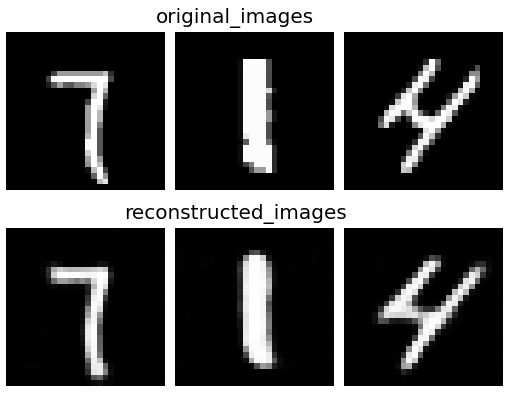
\includegraphics[height=0.8\textheight, width=\textwidth, keepaspectratio]{images/autoencoder/example_reconstruct.png}
    \caption{Image reconstruction with autoencoder trained on MNIST digits}
\end{figure}

\framebreak
\begin{figure}
    \centering
    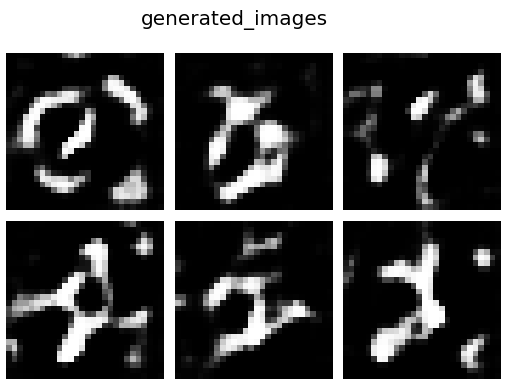
\includegraphics[height=0.8\textheight, width=\textwidth, keepaspectratio]{images/autoencoder/example_generative.png}
    \caption{Image generation with autoencoder trained on MNIST digits. Encoding vector sampled from latent space $Z$ and the passed to decoder.}
\end{figure}

\end{frame}